\documentclass[
  11pt,
  letterpaper,
   addpoints,
   answers
  ]{exam}

\usepackage[utf8]{inputenc}
\usepackage{../exercise-preamble}
\usepackage{float}
% TikZ libraries needed for `right=.. of ..` and coordinate math
\usetikzlibrary{positioning,calc,arrows,arrows.meta}
% Alias de seguridad por si se escribe 'ikzstyle' por error
\let\ikzstyle\tikzstyle

\begin{document}

\noindent
\begin{minipage}{0.47\textwidth}

\includegraphics[width=\textwidth]{../fcfm_die}
\end{minipage}
\begin{minipage}{0.53\textwidth}
\begin{center} 
\large\textbf{Análisis de señales} (EL3203-2) \\
\large\textbf{Clase auxiliar 3} \\
\normalsize Prof.~Jorge Silva.\\
\normalsize Prof.~Aux.~Erik Sáez
\end{center}
\end{minipage}

\vspace{0.5cm}
\noindent
\vspace{.85cm}

\begin{questions}
%----------------------------
\question
Considere la familia de funciones exponenciales discretas:
\begin{equation}
  A = \left\{ (\gamma_a(n)) \in \mathbb{R}^{\mathbb{N}} : \gamma_a(n) = a^n u(n),\ 0 < a < 1 \right\}
\end{equation}
\begin{enumerate}
  \item Verifique que el impulso discreto $\delta(n)$ puede ser expresado punto a punto como:
  \begin{equation}
    \delta(n) = \gamma_a(n) - a\,\gamma_a(n-1)
  \end{equation}
  \item Del punto anterior, muestre que toda señal discreta $x(n) \in \mathbb{R}^{\mathbb{Z}}$ puede ser descompuesta como:
  \begin{equation}
    x(n) = \sum_{k=-\infty}^{\infty} c_k\,\gamma_a(n-k)
  \end{equation}
  \item Use las propiedades de linealidad e invariancia en el tiempo para expresar la salida $y(n) = \mathcal{T}[x(n)]$ en términos de la entrada $x(n)$ y la señal $g(n) = \mathcal{T}[\gamma_a(n)]$.
\end{enumerate}
%----------------------------
\question
\begin{enumerate}
  \item Determine la transformada de Fourier de las siguientes señales y gráfiquela en magnitud y fase:
\begin{align*}
  &\bullet\quad x(t) = \begin{cases}
    A \cdot e^{-a t} & t \geq 0 \\
    0 & t < 0
  \end{cases} \\
  &\bullet\quad x(t) = A \cdot e^{-a|t|}
\end{align*}

\item Determine los coeficientes de la serie de Fourier para la siguiente señal:
\begin{equation}
  x(t) = 1 + \sin(\omega_0 t) + 2\cos(\omega_0 t) + \cos\left(2\omega_0 t + \frac{\pi}{4}\right)
\end{equation}
\end{enumerate}
%----------------------------
\begin{solution}
  a
\end{solution}
%----------------------------
\question Para la función sinusoidal rectificada mostrada en la figura \ref{fig:aux3_1}, calcule los coeficientes de la serie de Fourier , ademas verifique el cumplimiento del teorema de Parseval.
\begin{figure}[H]
    \centering
    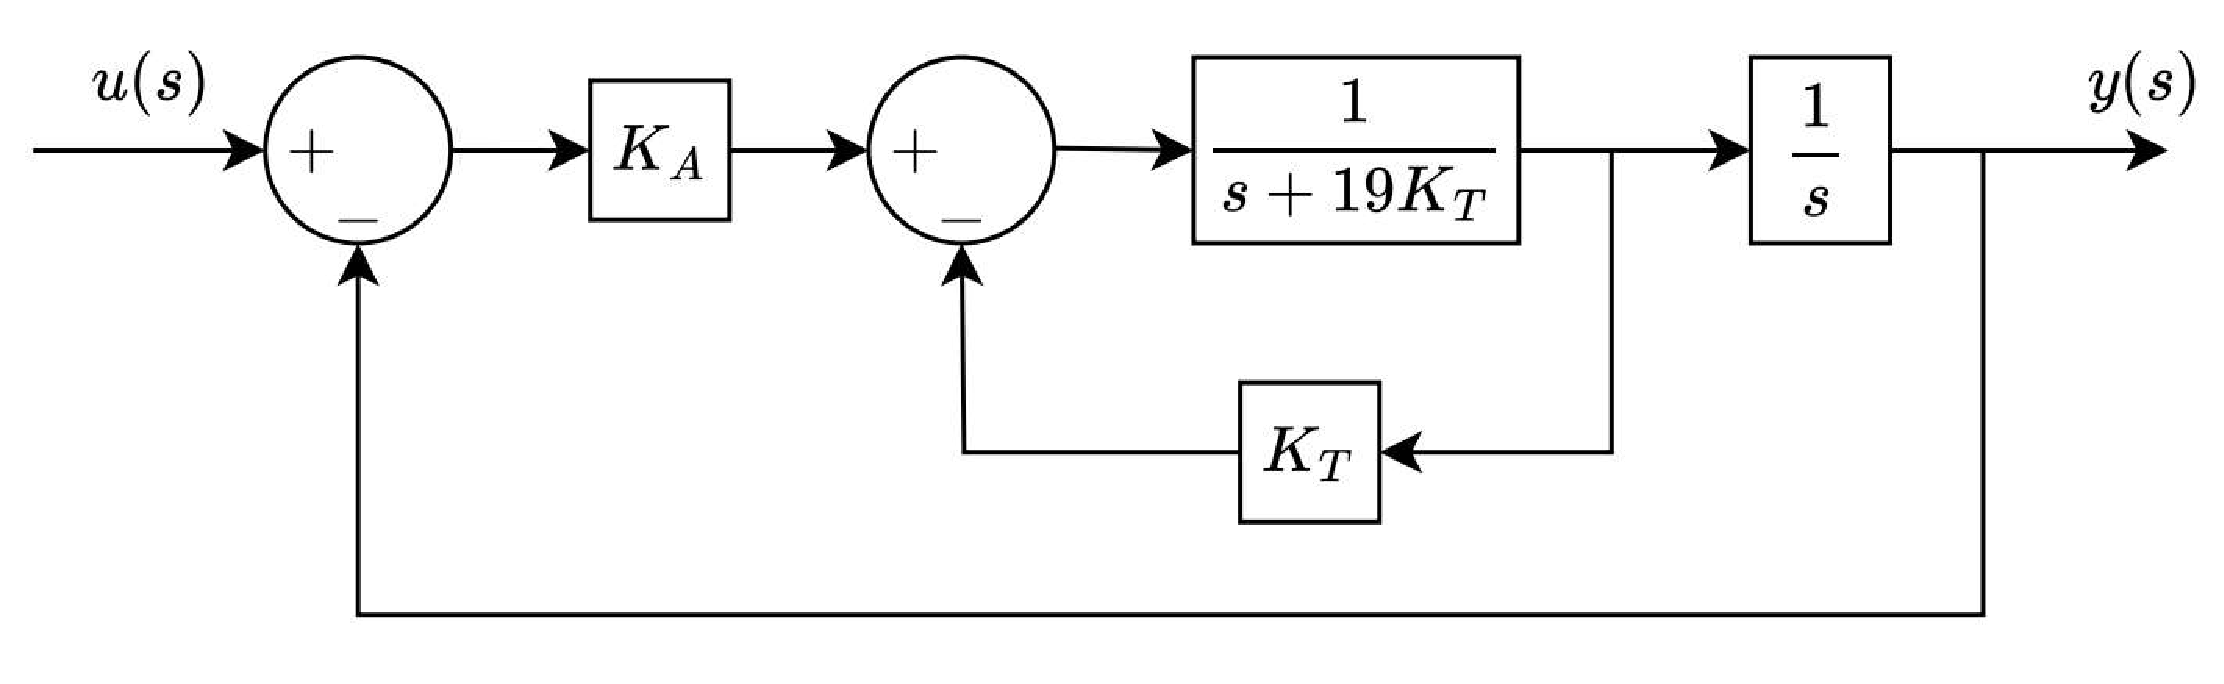
\includegraphics[width=0.6\textwidth]{Auxiliar_3_1}
    \caption{Función sinusoidal rectificada}
    \label{fig:aux3_1}
\end{figure}
%----------------------------
\begin{solution}
Los resultados obtenidos por Joseph Fourier nos indican que toda señal $x(t)$ continua y $T$-periódica, con $T > 0$, puede ser descrita como una serie de senos y cosenos ponderados según su componente frecuencial.

Formalmente, podemos definir una familia de funciones armónicas y $T$-periódicas dada por
\begin{equation}
  S_T := \left\{ \psi_k(t) = \left( e^{j \frac{2\pi}{T} k t} \right)_{t \in \mathbb{R}}\ :\ k \in \mathbb{Z} \right\}
\end{equation}

Con ello, se define la \textbf{ecuación de síntesis} como aquella que nos permite sintetizar o reconstruir la señal original $x(t)$ a partir de sus componentes frecuenciales $\frac{2\pi}{T}k$ y de sus coeficientes $c_k$ asociados:
\begin{equation}
  x(t) = \sum_{k=-\infty}^{\infty} c_k \cdot \psi_k(t)
\end{equation}
\begin{center}
  	extit{Ecuación de síntesis}
\end{center}

Complementariamente, se define la \textbf{ecuación de análisis} como aquella que nos permite analizar o evaluar el aporte de cada componente frecuencial $\frac{2\pi}{T}k$ en la señal calculando su coeficiente $c_k$:
\begin{equation}
  c_k = \frac{1}{T} \langle \psi_k(t), x(t) \rangle = \frac{1}{T} \int_{t_0}^{t_0+T} x(t) e^{-j \frac{2\pi}{T} k t} \, dt
\end{equation}
\begin{center}
  	extit{Ecuación de análisis}
\end{center}
\end{solution}
%----------------------------
\question Dadas dos señales $f(t)$ y $g(t)$ con coeficientes de Fourier $c_k$ y $d_k$, respectivamente, encuentre los coeficientes de Fourier de la señal $y(t) = f(t)
\end{questions}
\end{document}